\documentclass{article}

\usepackage{amssymb}
\usepackage{titlesec}
\usepackage{cancel}
\usepackage{enumerate}
\usepackage{multirow} % row merging in tables

\usepackage[utf8]{inputenc}
\usepackage[fleqn]{amsmath}
\usepackage{mathtools} % prettier set notation

\usepackage{multicol} % double column pages or more
\setlength\columnsep{20pt} % the default columnsep for all pages

% Better math
\usepackage{bm} % bold and italicize math
\usepackage{siunitx} % SI units with \si{...}

\usepackage[none]{hyphenat} % no line breaking on words
\usepackage[thinlines]{easytable} % better tables with row spacing

% Custom named colors
\usepackage[dvipsnames]{xcolor}
\definecolor{body}{HTML}{555555}
\definecolor{background}{HTML}{FFFFFF}

% Better tables
\usepackage{tabularx} % deprecated - use tabularrray instead - fit columns to width with \tabularx{\linewidth}{X}
\renewcommand{\arraystretch}{1.25}
\usepackage{arydshln} % dashed lines in tables
\newcolumntype{Y}{>{\centering\arraybackslash}X} % centered tabularx X columns with Y
\usepackage{tabularray} % modern table typesetting, superseding tabularx

% Better fonts
\usepackage{arev}
\usepackage[sfdefault]{inter}
\usepackage[T1]{fontenc}

% Better code formatting
\usepackage{listings}
\newcommand{\code}[1]{\texttt{#1}}
\lstset{
    mathescape,
    basicstyle=\small\fontfamily{lmvtt}\selectfont,
    numbers=left,
    numberstyle=\tiny,
    frame=tb,
    tabsize=4,
    columns=fullflexible,
    showstringspaces=false,
    showtabs=false,
    keepspaces,
    commentstyle=\color{red},
    keywordstyle=\color{blue}
}

% Insert images
\usepackage{graphicx}
\graphicspath{ {./images/} }

\usepackage{geometry}
\geometry{a4paper, portrait, margin=0.4in, top=0.7in}

\usepackage{fancyhdr}
\pagestyle{fancy}
\fancyhf{}
\lhead{CM1102 --- Chemistry -- The Central Science}
\rhead{Page \thepage}
\setlength{\headheight}{2em}
\renewcommand{\headrulewidth}{2pt}

\renewcommand{\labelenumii}{\theenumii}
\renewcommand{\theenumii}{\theenumi.\arabic{enumii}.}
\renewcommand{\labelenumiii}{\theenumiii}
\renewcommand{\theenumiii}{\theenumii\arabic{enumiii}.}

\setlength{\parindent}{0cm}
\setlength{\parskip}{0.7em}
\setlength{\abovedisplayskip}{0pt}
\setlength{\belowdisplayskip}{0pt}
\setlength{\abovedisplayshortskip}{0pt}
\setlength{\belowdisplayshortskip}{0pt}
\setlength{\mathindent}{0pt} % no indent for all math (including the align) environemnts

\titlespacing\part{0pt}{12pt plus 4pt minus 2pt}{0pt plus 2pt minus 2pt}
\titlespacing\section{0pt}{5pt plus 2pt minus 2pt}{0pt plus 2pt minus 2pt}
\titlespacing\subsection{0pt}{4pt plus 2pt minus 2pt}{-1pt plus 2pt minus 2pt}
\titlespacing\subsubsection{0pt}{3pt plus 2pt minus 2pt}{0pt plus 2pt minus 2pt}

\usepackage{etoolbox}
\newcommand{\zerodisplayskips}{%
  \setlength{\abovedisplayskip}{0pt}%
  \setlength{\belowdisplayskip}{0pt}%
  \setlength{\abovedisplayshortskip}{0pt}%
  \setlength{\belowdisplayshortskip}{0pt}}
\appto{\normalsize}{\zerodisplayskips}
\appto{\small}{\zerodisplayskips}
\appto{\footnotesize}{\zerodisplayskips}

% Remove vertical spacing around verbatim
\makeatletter
\preto{\@verbatim}{\topsep=-4pt \partopsep=0pt}
\makeatother

% Horizontal lines across a page
\newcommand{\pageline}[1]{\par\noindent\rule{\textwidth}{#1}}

% Proper double quotes
\newcommand{\quoted}[1]{\textquotedblleft{#1}\textquotedblright}

% Unordered list modifications
% Remove enumerate spacing with [leftmargin=*]
\usepackage{enumitem}
\setlist{nolistsep} % remove spacing in and around lists
\setlist[itemize]{leftmargin=*} % remove natural first level indent
\renewcommand{\labelitemi}{\textsc{--}} % change first level bullet to --

% Drawing trees
\usepackage[linguistics]{forest}

% Writing chemical formula and equations
\usepackage{mhchem}

% Drawing electronic configuration diagrams
% https://tex.stackexchange.com/questions/372581/atomic-electronic-configuration-with-small-boxes
\newcommand*\up{\fbox{$\mathord\upharpoonleft\phantom{\downharpoonright}$}}%
\newcommand*\dwn{\fbox{$\mathord\downharpoonleft\phantom{\upharpoonright}$}}%
\newcommand*\updwn{\fbox{$\upharpoonleft\downharpoonright$}}%
\newcommand*\emp{\fbox{$\phantom{\downharpoonright}\phantom{\downharpoonright}$}}%
\newcommand{\electron}[2]{{%
        \setlength\tabcolsep{0pt}% remove extra horizontal space from tabular
%       \setlength\fboxrule{0.2pt}% uncomment for original line width
        \begin{tabular}{c}
            \fboxsep=0pt\fbox{\fboxsep=3pt#2}\\[2pt]
            #1
        \end{tabular}%
}}

\title{\vspace{-1cm}\textbf{CM1102 \\[0.25em] Chemistry -- The Central Science} \\[2em] \Large AY2022/23 Semester 1 \\[1em]}
\author{Notes by Jonathan Tay}
\date{Last updated on \today}

\color{body}
\pagecolor{background}
\begin{document}
    \pagenumbering{gobble} % remove page numbering for content pages
    \maketitle
    \pageline{1.5pt}
    \renewcommand{\baselinestretch}{0.75}\normalsize
    \tableofcontents
    \renewcommand{\baselinestretch}{1.1}\normalsize
    \pageline{1.5pt}

    \newpage
    \pagenumbering{arabic} % re-add page numbering
    \begin{multicols*}{2}
        \part{Environment}
        \section{Light}
\textbf{Light} is a form of energy that consists of oscillating \emph{electric} and \emph{magnetic}
fields, perpendicular to each other.

\begin{tabularx}{\linewidth}{|l|X|l|} \hline
    \multicolumn{3}{|c|}{$c = \lambda \nu$} \\ \hline
    & \textbf{value} & \textbf{unit} \\ \hline
    $c$ & speed of light $= 2.9979 \times 10^8$ & m/s \\ \hdashline
    $\lambda$ & wavelength & m \\
    $\nu$ & frequency & $s^{-1}$ or Hz \\ \hline
\end{tabularx}

\subsection{Wave-particle Duality of Light}

Due to the wave nature of light, light waves that are \textit{in phase} undergo 
\textbf{constructive interference}.

Light waves that are \textit{out of phase} undergo \textbf{destructive interference} 
--- cancelling out each other.

Due to the particle nature of light, when an object is heated, 
it emits electromagnetic radiation known as \textbf{blackbody radiation}.

The wavelength of light emitted changes as the temperature of the object increases.

\begin{tabularx}{\linewidth}{|l|X|l|} \hline
    \multicolumn{3}{|c|}{$E = h \nu$} \\ \hline
    & \textbf{value} & \textbf{unit} \\ \hline
    $E$ & energy & J \\ \hdashline
    $h$ & Planck's constant $= 6.626 \times 10^{-34}$& J/s \\
    $\nu$ & frequency & $s^{-1}$ or Hz \\ \hline
\end{tabularx}

Putting the two equations above together, we can interconvert between \textit{energy}, 
\textit{frequency}, and \textit{wavelength}.

\begin{tabularx}{\linewidth}{|l|X|l|} \hline
    \multicolumn{3}{|c|}{$E = \frac{hc}{\lambda}$} \\ \hline
    & \textbf{value} & \textbf{unit} \\ \hline
    $E$ & energy & J \\ \hdashline
    $h$ & Planck's constant $= 6.626 \times 10^{-34}$& J/s \\
    $c$ & speed of light $= 2.9979 \times 10^8$ & m/s \\
    $\lambda$ & wavelength & m \\ \hline
\end{tabularx}

\subsection{Photoelectric Effect}
Electrons can only be ejected from a surface if incoming \textbf{photons} transfer
sufficient energy to the atoms on the metal surface.

\textbf{Electron-volt} (eV) is the amount of \textit{kinetic energy} gained by a single
electron accelerating from rest though an electric potential difference of 1 volt in vacuum.

\begin{tabularx}{\linewidth}{|Y|} \hline
    $1 \; \si{\electronvolt} = 1.602 \times 10^{-19}$ \si{\joule} \\ \hline
\end{tabularx}

\begin{tabularx}{\linewidth}{|l|X|l|} \hline
    \multicolumn{3}{|c|}{$h \nu = \Phi + \text{KE}_{\text{max}}$} \\ \hline
    & \textbf{value} & \textbf{unit} \\ \hline
    $h$ & Planck's constant \par $= 6.626 \times 10^{-34}$& J/s \\
    $\nu$ & frequency & $s^{-1}$ or Hz \\ \hdashline
    $\Phi$ & work function of the metal & eV \\
    $\text{KE}_{\text{max}}$ & maximum kinetic energy of the ejected electron & eV \\ \hline
\end{tabularx}

Note that $\text{KE}_{\text{max}}$ \textit{cannot be negative}, so its minimum value is 0.

\subsection{Solar Spectrum}
The \textbf{electromagnetic spectrum} comprises of, in increasing energy:
\begin{enumerate}
    \item radio waves,
    \item microwaves,
    \item infrared,
    \item visible,
    \item ultraviolet,
    \item X-rays,
    \item gamma ($\gamma$) rays,
\end{enumerate}

White light disperses into a continuous spectrum in the visible spectrum.

However, sunlight is \emph{not continuous} --- there are \emph{dark lines} in
the \textbf{solar spectrum} due to the composition of the sun and the Earth's atmosphere.

\subsubsection{Aside: Spectroscopy}

\emph{The study of the interaction of \emph{electromagnetic radiation}
with \emph{matter} to obtain information about the identity and structure of substances.}

\textbf{Absorption spectroscopy} reveals that a colored object reflects light of that color
and absorbs light of the \textit{opposite color}.

\subsubsection{Emission Spectrums}
Energy can excite electrons of atoms from their \textbf{ground state} to an \textbf{excited state}.

In the excited state, electrons have higher energy, and when electrons are relaxed to their
ground state, their energy is released as light.

Therefore, the dark lines in the solar spectrum occur due to the absorption of energy
by the atoms in the sun's atmosphere.

\subsubsection{Rydberg Formula}
\emph{Used to calculate the wavelengths of a spectral line in hydrogenic species, i.e. H, $\text{He}^{\text{+}}$, $\text{Li}^{\text{2+}}$, etc.}

It generalizes the Balmer series ($n = 2$) for the visible region, the Lyman series ($n = 1$)
for the UV region, and the Paschen series ($n = 3$) for the IR region.

\begin{tabularx}{\linewidth}{|l|X|l|} \hline
    \multicolumn{3}{|c|}{$\frac{1}{\lambda} = R_H \left( \frac{1}{{n_1}^2} - \frac{1}{{n_2}^2} \right)$} \\ \hline
    & \textbf{value} & \textbf{unit} \\ \hline
    $\lambda$ & wavelength of light emitted & m \\ \hdashline
    $R_H$ & Rydberg constant $= 1.096776 \times 10^7$ & $\si{\per\metre}$ \\
    $n_1$ & final electron state (lower energy) $< n_2$ & \code{int} \\
    $n_2$ & initial electron state (higher energy) & \code{int} \\ \hline
\end{tabularx}
        \section{Energy Levels}

In the Bohr model, electrons are allowed only in certain circular orbits around the nucleus,
which give rise to the \textbf{principal quantum numbers} of $n$.

Therefore, the energy levels in atomic structures are \emph{quantized},
and the energy levels associated with each electron orbit has a fixed value,
hence the term \textbf{quantized energy level}.

\begin{tabularx}{\linewidth}{|l|X|l|} \hline
    \multicolumn{3}{|c|}{$E_n = -\frac{2 \pi^2 m_e e^4}{n^2 h^2}$} \\ \hline
    & \textbf{value} & \textbf{unit} \\ \hline
    $E_n$ & energy level & J \\ \hdashline
    $m_e$ & electron mass $= 9.1094 \times 10^{-31}$ & \si{\kilo\gram} \\
    $e$ & electron charge $= 1.602 \times 10^{-19}$& \si{\coulomb} \\
    $n$ & principal quantum number & \code{int} \\
    $h$ & Planck's constant $= 6.626 \times 10^{-34}$& \si{\joule \cdot \sec} \\ \hline
\end{tabularx}

Since the only variable is $n$, the equation is generalizable:

\begin{tabularx}{\linewidth}{|Y|} \hline
    $E_n \approxeq -2.18 \times 10^{-18} \left( \frac{1}{n^2} \right)$ \si{\joule} \\ \hline
    $E_n \approxeq -13.6 \left( \frac{1}{n^2} \right)$ \si{\electronvolt} \\ \hline
\end{tabularx}

The \textbf{ground state} of electrons, $n = 1$, has the lowest energy level and the most stable.

The \textbf{excited states} have values of $n > 1$.

The energy required to excite an electron from the ground state to an excited state 
$\Delta E = E_{\text{final}} - E_{\text{initial}}$ can be determined using the $E_n$ formula above.

If $\Delta E > 0$, this is known as an \textbf{absorption} (or excitation) process,
going from a lower energy state to a higher energy state.

Conversely, if $\Delta E < 0$, this is known as an \textbf{emission} (or relaxation) process,
going from a higher energy state to a lower energy state, which releases energy.

The \textbf{ionization continuum} occurs as $n \rightarrow \infty, E_n \rightarrow 0$,
such that energy levels are no longer quantized.

The \textbf{ionization energy} is the minimum energy required to remove one electron from
a gaseous atom or molecule.

In the case of hydrogen, $\Delta E = E_\infty - E_1 = + 13.6 \si{\electronvolt}$.

However, this only applies to 1-electron systems, as we otherwise need to account for
electron-electron repulsion, which requires taking into account the nuclear charge, $Z^2$:

\begin{tabularx}{\linewidth}{|Y|} \hline
    $E_n \approxeq -2.18 \times 10^{-18} \left( \frac{Z^2}{n^2} \right)$ \si{\joule} \\ \hline
    $E_n \approxeq -13.6 \left( \frac{Z^2}{n^2} \right)$ \si{\electronvolt} \\ \hline
\end{tabularx}
        \section{Atomic Structure}
Electrons, and all matter, behave like waves, which can undergo constructive and destructive
interference.

\begin{tabularx}{\linewidth}{|l|X|l|} \hline
    \multicolumn{3}{|c|}{$\lambda = \frac{h}{mv}$} \\ \hline
    & \textbf{value} & \textbf{unit} \\ \hline
    $\lambda$ & De Broglie wavelength & m \\ \hdashline
    $h$ & Planck's constant $= 6.626 \times 10^{-34}$& J/s \\
    $m$ & particle mass & \si{\kilo\gram} \\
    $v$ & particle velocity & \si{\metre\per\sec}\\ \hline
\end{tabularx}

By \textbf{Heisenberg's uncertainty principle}, it is impossible to know the precise position
of electrons in an atom.

\subsection{Quantum Mechanical Model}
A \textbf{wave equation} describes the behavior of a specific electron in an atom.

The solution to the wave equation is called a \textbf{wave function} ($\psi$), 
or an \textbf{orbital} --- the space boundary where there is a 95\% chance of finding the electron.

$|\psi|^2$ is proportional to the \emph{probability density} of an electron being found in 3D space.

The position of an electron could be described using \textit{Cartesian coordinates}, using the wave
equation $\psi(x, y, z)$.

Alternatively, using \textit{spherical coordinates}, $\psi(r, \theta, \phi)$:

\begin{tabularx}{\linewidth}{|l|X|l|} \hline
    \multicolumn{3}{|c|}{$\psi(r, \theta, \phi) = \mathbf{R}(r) \times \mathbf{Y}(\theta, \phi)$} \\ \hline
    & \textbf{value} & \textbf{unit} \\ \hline
    $\mathbf{R}(r)$ & \textbf{radial wave function} & -- \\
    $r$ & distance of the electron from the nucleus & -- \\ \hdashline
    $\mathbf{Y}(\theta, \phi)$ & \textbf{angular wave function} & -- \\
    $\theta$ & vertical angle perpendicular to the $x$-$y$ plane & -- \\
    $\phi$ & angle on the $x$-$y$ plane & -- \\ \hline
\end{tabularx}

\textbf{Radial nodes} are regions where the \textit{radial} component of the wave function passes through 0
--- appearing as a \emph{nodal sphere} expanding from the center, where no electrons are found.

\textbf{Angular nodes} are regions where the \textit{angular} component of the wave function passes through 0
--- appearing in the \emph{x-y plane} where no electrons are found.

In orbital diagrams, the regions corresponding to positive values of the wave function are shaded,
while the regions corresponding to negative values are not.

\subsubsection{Radial Distribution Function (RDF)}
\begin{tabularx}{\linewidth}{|l|X|l|} \hline
    \multicolumn{3}{|c|}{$RDF: 4 \pi r^2 \cdot \mathbf{R}(r)^2$ } \\ \hline
    & \textbf{value} & \textbf{unit} \\ \hline
    $4 \pi r^2$ & surface area of a sphere & -- \\
    $\mathbf{R}(r)$ & radial wave function & -- \\ \hline
\end{tabularx}

\vspace*{1em}
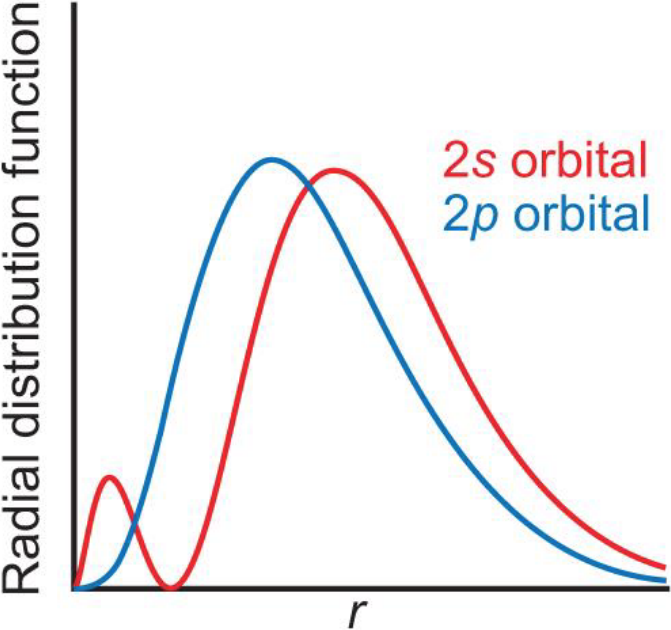
\includegraphics[width=\linewidth/2]{rdf}

The maximum value of the RDF (i.e. the peak) is the most probable distance of the electron
from the nucleus.

Even though the larger peak of the $2p$ orbital is closer than that of the $2s$ orbital,
the $2s$ orbital has a higher energy level than the $2p$ orbital due to the \textbf{penetration}
from the smaller peak.

Therefore, within shells of the same quantum number, orbital energy increases as follows:
 $s < p < d < f$.

 Radial nodes can be counted from the $x$-intercepts, so from the diagram above,
 the $2s$ orbital has 1 radial node, while the $2p$ orbital has none.

 \subsubsection{Quantum Numbers}
 \begin{tabularx}{\linewidth}{|l|X|X|} \hline
    \multicolumn{3}{|c|}{$nl_{m_l}$, e.g. $2p_z$} \\ \hline
    & \textbf{value} & \textbf{range} \\ \hline
    $n$ & \textbf{principal} QN & 1, 2, 3, \dots \\
    $l$ & \textbf{magnetic} QN & 0, 1, \dots, $n-1$ \\
    $m_l$ & \textbf{orbital angular momentum} QN & $-l, \dots, 0, \dots, +l$ \\ \hline
\end{tabularx}

The principal QN relates to the \textit{size} and \textit{energy} of the orbital --- higher principal QNs
have larger orbitals with higher energy levels.

The magnetic QN relates to the \textit{shape} of the orbital.

The orbital angular momentum QN relates to the \textit{orientation} of the orbital.

\begin{tabularx}{\linewidth}{|Y|c|} \hline
    number of angular nodes & $l$ \\ \hline
    number of radial nodes & $n - l - 1$ \\ \hline
\end{tabularx}
    \end{multicols*}
\end{document}